\section{\index{ODMR}{ODMR}}\label{ODMR}
Optically detected magnetic resonance, specifically continuous wave optically detected magnetic resonance will be the read-out mechanism discussed in this work. This is not necessarily the most sensitive mechanism for any given system, but remains popular due to the very simple implementation. 

The process is to measure the photoluminescence of the spin polarised sample whilst sweeping the driving field to find where the Rabi oscillations occur. When the change of photoluminescence is at a peak, the Rabi frequency is exactly the energy difference between the two spin sub-levels. The energy of and energy difference between the spin sub-levels is dependent on the magnetic and electric field, temperature, pressure and strain. 

\begin{figure}[h]
    \begin{center}
        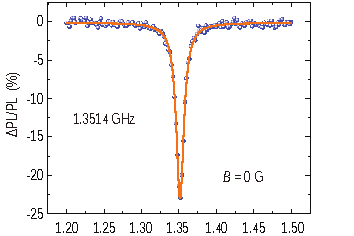
\includegraphics[width=0.5\textwidth]{figures/ODMR.pdf}
    \end{center}
    \caption{
        CW-ODMR spectra for a PL6 defect with $\vec{B} = 0$. Blue dots show data from experiment, the orange line is a Lorentzian fit. Adapted from Li et al.}\label{fig:}
%  CW-ODMR
% spectra in the zero magnetic field. The blue dots are the experimental raw data, and the orange line is the corresponding Lorentzian fitting centred
% at 1.3514 GHz.
    % \cite{Li2021}
    % \todo[inline, color=ediblue]{Write caption}
\end{figure}


Determination of how these physical characteristics influence the change in ODMR spectra is the topic of this work. 


% The results suggest that magnetic field sensing sensitivity can be greatly improved for the optimized laser and microwave power range.
% \cite{PhysRevB.101.064102}


% We measure increased photoluminescence from divacancy ensembles by up to three orders of magnitude using near-ultraviolet excitation, depending on the substrate, and without degrading the electron spin coherence time.
% \cite{Wolfowicz2017}


